\documentclass[addpoints,a4]{exam} % use parameter answers to see solutions
\usepackage[utf8]{inputenc}
\usepackage{times}
\usepackage{hyperref}
\usepackage{enumitem}
\usepackage{graphicx}
\usepackage{amsmath}
\usepackage{amssymb}
\usepackage{tikz}
\usepackage{algorithm2e}
\graphicspath{ {figs/} }
\usepackage{upquote} % for normal looking single quote inside verbatim
%\usepackage{resizebox}
%\setlength{\parskip}{2px}%
%\usetikzlibrary{graphdrawing.trees}

\usepackage{pythonhighlight}



\usepackage[top=2.6cm,left=2.5cm,right=2.5cm]{geometry}


\pagestyle{headandfoot}
\runningheader{
    \normalsize\bfseries Full name:\enspace\makebox[2.2in]{\hrulefill} \normalsize\bfseries
    Student ID/Date of birth:\enspace\makebox[2in]{\hrulefill}
}
{}
{}
\firstpagefooter{}{}{}
\runningfooter{}{\thepage}{}




  
\qformat{\large{\textbf{Question \thequestion: \thequestiontitle}}\quad (\totalpoints \,\,points)\hfill}


% https://tex.stackexchange.com/questions/171991/exam-documentclass-question-title-grading-table#172036
\usepackage{etoolbox}
\makeatletter
\patchcmd{\questions}
  {\def\@currentlabel{\thequestiontitle}}
  {\def\@currentlabel{\thequestion}}
  {}
  {}
\makeatother

\hypersetup{
    colorlinks,
    citecolor=black,
    filecolor=black,
    linkcolor=black,
    urlcolor=blue
}

\title{
	{\large Write your full name and your student ID/date of birth on top of all the pages}\\[2cm]
	
	\textbf{Mock Exam}\\
    Introduction to Data Science and Programming
    }

\date{Month Day, Year}

\author{}

\begin{document}
\maketitle

\begin{center}
\pointtable[v][questions]\\[30pt]

\end{center}




\clearpage
%Here, the questions begin
\begin{questions}
\titledquestion{Data Structures}\vspace{30pt} Consider the following list of different lamps from an inventory, listing for each type of lamp the name and stock (how many are available). Suppose this list data structure contains $n$ entries.
\begin{python}
stock_lamps = [
	("henningsen", 87),
	("panton", 53),
	("poulsen", 8),
	..., # the list continues here
	("leklint", 35)]

\end{python}
\begin{parts}
\part[5] Say we need to change the stock for one of the lamps. This lamp is identified by the string, say, \verb^lamp = "nuura"^ - we do not know its position in the list. In the worst case scenario, explain how long it would take, in relation to $n$, to perform this operation with this data structure? What about the best case scenario?
\begin{solution}[\stretch{0.5}]
Worst case scenario is that the lamp we are looking for is the last tuple in both of the lists. In that case we have to look through the whole list, that is $n$ operations, i.e., $O(n)$. The best case is that it's the first in both lists, then we get 2 operations which is $O(1)$.
\end{solution}
\part[5] Which Python data structure would be most efficient out of the data structures you learned to carry out the same task (without importing any library)? Explain, i.e.~give the best and worst case amount of time in relation to $n$.
\begin{solution}[\stretch{0.5}]
A dictionary is most efficient since it can access the count for a specific word in constant time if we set the key to be the lamp string and the value to be the count. Both best and worst case are $O(1)$ (if we exclude rare ``amortized worst cases'').
\end{solution}
\end{parts}



\clearpage
\titledquestion{Variables and Program Flow} 
\begin{parts}
\part
Consider the block of Python code below.
\begin{python}
i = 100
mylist = []
while True:
    modulo121 = i % 121
    if modulo121 == 0:
        mylist.append(i)
    i += 1
    if i > 3000:
        break
\end{python}

\begin{subparts}
\subpart[2] Describe in your own words what this while-loop does, and what \verb+mylist+ will contain after you run the code. You don't need to give the exact numbers; a short description is sufficient.
\begin{solution}[\stretch{1}]
It contains all integers between 100 and 3000 that are divisible by 121.
\end{solution}
\subpart[3] Write an implementation for the same functionality, i.e. producing a list \verb+mylist+ with the same content, with a for loop instead of a while loop.
\begin{solution}[\stretch{1.7}]
\begin{python}
mylist = []
for i in range(100,3000):
    modulo121 = i % 121
    if modulo121 == 0:
        mylist.append(i)
\end{python}
\end{solution}
\end{subparts}

\part[2] In the code above, after the while-loop finishes, the variable \verb+mylist+ contains 24 items.\\
Now instead, consider the block of Python code below.
\begin{python}
i = 1
longlist = []
while True:
    modulo5 = i % 5
    if modulo5 == 0:
        longlist.append(i)
    i += 1
\end{python}
Can you estimate the length of \verb+longlist+? Give a very short explanation.
\begin{solution}[\stretch{0.5}]
No, it will fill up indefinitely as the while loop will never stop.
\end{solution}

\part Consider the block of Python code below.
\begin{python}
s1 = True
s2 = False
s3 = True or False
s4 = True and False
all_statements = [s1, s2, s3, s4]
sum_statements = sum(all_statements)
long_statement = (s1 and s3) and (s3 or s2) and (s2 or s4)
\end{python}
\begin{subparts}
\subpart[2] What is the variable type and the value of \verb+sum_statements+?
\begin{solution}[\stretch{0.5}]
int, 2
\end{solution}
\subpart[1] What is the boolean value of \verb+long_statement+?
\begin{solution}[\stretch{0.5}]
False
\end{solution}
\end{subparts}
\end{parts}


\clearpage
\titledquestion{Function Analysis} Consider the block of Python code below.
\begin{python}
def isletter(character):
    letters = ["a","b","c","d","e","f","g","h","i","j","k","l","m","n","o","p","q","r","s","t","u","v","w","x","y","z"]
    if character in letters:
        return True 
    return False

def myfunction(s):
    wordlist = []
    word = ""
    for i in range(len(s)): 
        character = s[i]
        mode = len(wordlist) % 2  # modulo. The first mode will be 0.
    
        if isletter(character):
            if mode == 0: 
                word = word + character
            elif mode == 1:
                word = word + "?" 
            else:
                word = word + "%" 
        elif character == ",":
            wordlist.append(word) # adding word to wordlist
            word = "" # starting next word

    if word != "":  # don't forget the last word
        wordlist.append(word)
    
    return wordlist

print(myfunction("*h8/ap_9py,ate*,n3e*_w,oh,y9ea/r"))
\end{python}
\begin{parts}
\part[3] What does the code print out?
\begin{solution}[\stretch{1}]
\verb+['happy', '???', 'new', '??', 'year']+
\end{solution}
\part[5] Describe in your own words what the $\mathrm{myfunction()}$ function does to a string input? 
\begin{solution}[\stretch{3}]
It splits it into words separated by commas, stored in a list. Non-letter characters are ignored. Letters in every second word are replaced by question marks.
\end{solution}
\part[2] Which two consecutive lines of code inside the function $\mathrm{myfunction()}$ can be deleted without affecting the function's output?
\begin{solution}[\stretch{2}]
\begin{python}
            else:
                word = word + "%" 
\end{python}
\end{solution}
\end{parts}



\clearpage
\titledquestion{Induction}[10] 
Consider the equation below.
\begin{equation*}
\sum_{i=1}^{n}i^3 = \frac{1}{4}n^2(n+1)^2
\end{equation*}
Prove, using induction, that the equation holds for all $n \geq 1$. Explicitly state the base case and the inductive assumption.
\begin{solution}[\stretch{0.5}]
The equality holds for the base case $n=1$:
\begin{eqnarray*}
\sum_{i=1}^{1}i^3 & = & \frac{1}{4}1^2(1+1)^2\\
1 & = & \frac{1}{4}4 \quad = \quad 1
\end{eqnarray*}
Let us assume it holds for $n=k$ (inductive assumption):
\begin{equation*}
\sum_{i=1}^{k}i^3 = \frac{1}{4}k^2(k+1)^2
\end{equation*}
We check that then it holds for $n=k+1$:
\begin{eqnarray*}
\sum_{i=1}^{k+1}i^3 & = & \frac{1}{4}(k+1)^2(k+2)^2
\end{eqnarray*}
It is true that $\sum_{i=1}^{k+1}i^3  =  \sum_{i=1}^{k}i^3 + (k+1)^3$. Using the inductive assumption in the left hand side, we show the following equality:
\begin{eqnarray*}
\frac{1}{4}k^2(k+1)^2 + (k+1)^3 & = & \frac{1}{4}(k+1)^2(k+2)^2 \qquad | :(k+1)^2 \\
\frac{1}{4}k^2 + (k+1) & = & \frac{1}{4}(k+2)^2 \qquad | \times 4 \\
k^2 + 4(k+1) & = & (k+2)^2 \\
k^2 + 4k + 4 & = & k^2 + 4k + 4 \quad\square
\end{eqnarray*}
\end{solution}


\clearpage
\titledquestion{Data Exploration} Consider the following data set with attributes and measurements about bicycle paths in Copenhagen.\\

\begin{tabular}{rrrrr}
pathID & width & flow  & priority & protected \\
104    & 180        & 2400  & 1        & 1         \\
105    & 120        & 3600  & 1        & 0         \\
106    & 158        & 8800  & 1        & 1         \\
201    & 178        & 10000 & 3        & 1         \\
202    & 162        & 4600  & 2        & 1         \\
203    & 220        & 8000  & 2        & 1         \\
204    & 220        & 7400  & 1        & 0         \\
205    & 240        & 7800  & 1        & 1         \\
301    & 186        & 4600  & 2        & 1         \\
302    & 140        & 12000 & 3        & 1         \\
303    & 180        & 4600  & 2        & 1         \\
304    & 182        & 9800  & 3        & 1         \\
305    & 168        & 8800  & 1        & 1      
\end{tabular}


\begin{parts}
\part[2] Which of the variables are quantitative?
\begin{solution}[\stretch{0.3}]
width, flow
\end{solution}

\part[3] Suppose you load the data into Python like this:
\begin{verbatim}
data = numpy.loadtxt("data.csv", skiprows=1, dtype="int")
\end{verbatim}

The company \emph{Hypercykelstier} is conducting a study on which of the bicycle paths could qualify as a ``hyper bicycle path''. A path qualifies as ``hyper'' if it is protected and if at least one of these two conditions hold: Its width must be at least 160 cm, or it must have priority 1. Create a mask that selects all paths that qualify as ``hyper'':
\begin{verbatim}
mask = (                  ) & ((                  )|(                  ))
\end{verbatim}
where \verb+data[mask,0]+ should return the qualified pathIDs.
\begin{solution}[\stretch{0.3}]
\begin{verbatim}
mask = (data[:, 4] == 1) & ((data[:, 1] >= 160) | (data[:, 3] == 1))
\end{verbatim}
\end{solution}

\part[5]
Calculate the five number summary for the flows over all paths that qualify as ``hyper'' and report their sorted flows. If a five number summary value falls between two data points, take the midpoint (average) between the two data points.
\begin{solution}[\stretch{1.5}]
Sorted weight values: 2400,  4600,  4600,  4600,  7800,  8000,  8800,  8800,  9800,
       10000\\
Five number summary: min: 2400, $Q_1$: 4600, median: 7900, $Q_3$: 8800, max: 10000
\end{solution}
\end{parts}




\clearpage
\titledquestion{Visual Data Reporting}[10] Consider the data set \verb+data_hyper = data[mask]+, where \verb+data+ and \verb+mask+ are taken from the previous question.

Draw by hand as exactly as possible what the following code will output. You can use the two boxes below the code for \verb+axis1+ and \verb+axis2+. Draw all elements, including ticks, labels, titles, bars, scatterplot markers, at their correct locations. You do not need to get the colors right.
\begin{python}
import numpy as np
import matplotlib.pyplot as plt

categories, counts = np.unique(data_hyper[:, 3], return_counts=True)

fig, axes = plt.subplots(nrows=1, ncols=2, figsize=(9, 4))
axis1 = axes[0] 
axis2 = axes[1]

axis1.bar(categories, counts)
axis1.set_title("Priority")
axis1.set_xticks(categories)
axis1.set_xticklabels(["High", "Medium", "Low"])

axis2.scatter(data_hyper[:,2], data_hyper[:,1])
axis2.set_xlabel("Flow")
axis2.set_ylabel("Width");
\end{python}

\vspace{25px}
\begin{center}

\includegraphics[width=0.98\columnwidth]{box.png} % Example image
%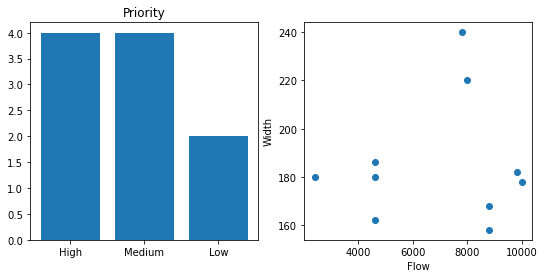
\includegraphics[width=0.98\columnwidth]{plotsolution.png} % Example image
\end{center}





\clearpage
\titledquestion{Network Metrics} Given the following network. 
\begin{center}
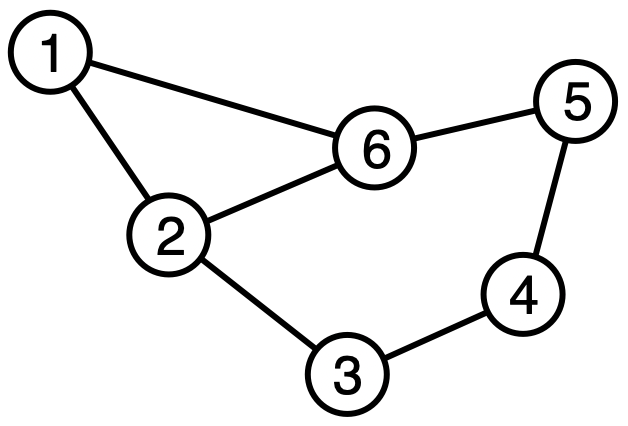
\includegraphics[width=0.30\columnwidth]{network.png} % Example image
\end{center}

%This question has several parts
\begin{parts}
\part[2] Calculate the degrees $k_1,k_2,\ldots,k_6$, and the average degree $\langle k \rangle$ of the network.
\begin{solution}[\stretch{2}]
$k_1=2, k_2=3, k_3=2, k_4=2,k_5=2,k_6=3,\langle k \rangle = \frac{2+3+2+2+2+3}{6} = \frac{14}{6}$
\end{solution}
%Equally distributes the available space
\part[3] Calculate the clustering coefficients $c_1$, $c_2$ and $c_3$ of nodes 1, 2 and 3.
\begin{solution}[\stretch{2}]
$c_1 = 1, c_2 = \frac{1}{3}, c_3 = 0$
\end{solution}


\part[4] Calculate the average path length $\ell$ and the diameter $D$.
\begin{solution}[\stretch{5}]
$\ell = \frac{(1+2+3+2+1)+(1+1+2+2+1)+(2+1+1+2+2)+(3+2+1+1+2)+(2+2+2+1+1)+(1+1+2+2+1)}{30} = \frac{9+7+8+9+8+7}{30} = \frac{48}{30}$ = 1.6, $D = 3$
\end{solution}

\part[1] If there is a cycle of length 5 then report one below, otherwise write ``No''.
\begin{solution}[\stretch{1}]
2,3,4,5,6,2
\end{solution}


\end{parts}



\clearpage
\titledquestion{Network Data Structure} For the network from the previous question:

\begin{parts}
\part[1]  Write down the adjacency matrix.
\begin{solution} [\stretch{2}] %Equally distributes the available space
$A = \begin{pmatrix}
0 & 1 & 0 & 0 & 0 & 1\\
1 & 0 & 1 & 0 & 0 & 1 \\
0 & 1 & 0 & 1 & 0 & 0 \\
0 & 0 & 1 & 0 & 1 & 0\\
0 & 0 & 0 & 1 & 0 & 1\\
1 & 1 & 0 & 0& 1 & 0
\end{pmatrix}$
\end{solution}

\part[1] Write down the edge list.
\begin{solution}[\stretch{2}]
$I = \begin{pmatrix}
1 \\ 1 \\ 2 \\ 3 \\ 4 \\ 5
\end{pmatrix}$, 
$J = \begin{pmatrix}
2 \\ 6 \\ 3 \\ 4 \\ 5 \\ 6
\end{pmatrix}$
\end{solution}

\part[1] Write down the adjacency list.
\begin{solution}[\stretch{1}]
$1 = \{2,6\}, 2 = \{1,3\}, 3 = \{2,4\}, 4 = \{3,5\}, 5 = \{4,6\}, 6=\{1,2,5\}$
\end{solution}

\part
\begin{subparts}
\subpart[4] Remove from the same network below two links to increase the graph distance $d_{1,6}$ between the nodes 1 and 6 from $d_{1,6}=1$ to $d_{1,6}=5$. Indicate in the figure below where you remove the links. \begin{center}
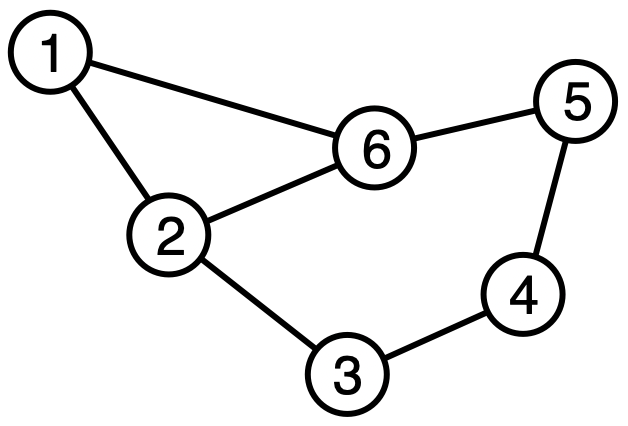
\includegraphics[width=0.30\columnwidth]{network.png} % Example image
%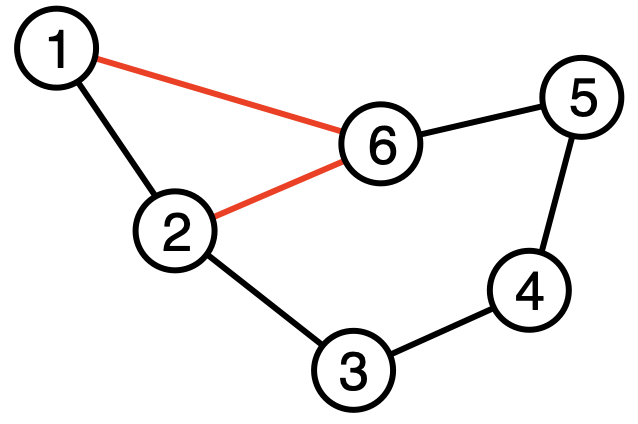
\includegraphics[width=0.30\columnwidth]{networksolution.png}
\end{center}
\subpart[3] For this new network: What is then the new average degree, and what is the new diameter?
\begin{solution}[\stretch{1}]
$\langle k \rangle_\mathrm{new} = \frac{1+2+2+2+2+1}{6} = \frac{10}{6}=1.67$, $D = 5$
\end{solution}


\end{subparts}
\end{parts}




\clearpage
\titledquestion{Graph Algorithms}
Consider the following undirected weighted graph.
\begin{figure}[ht!]
\centering
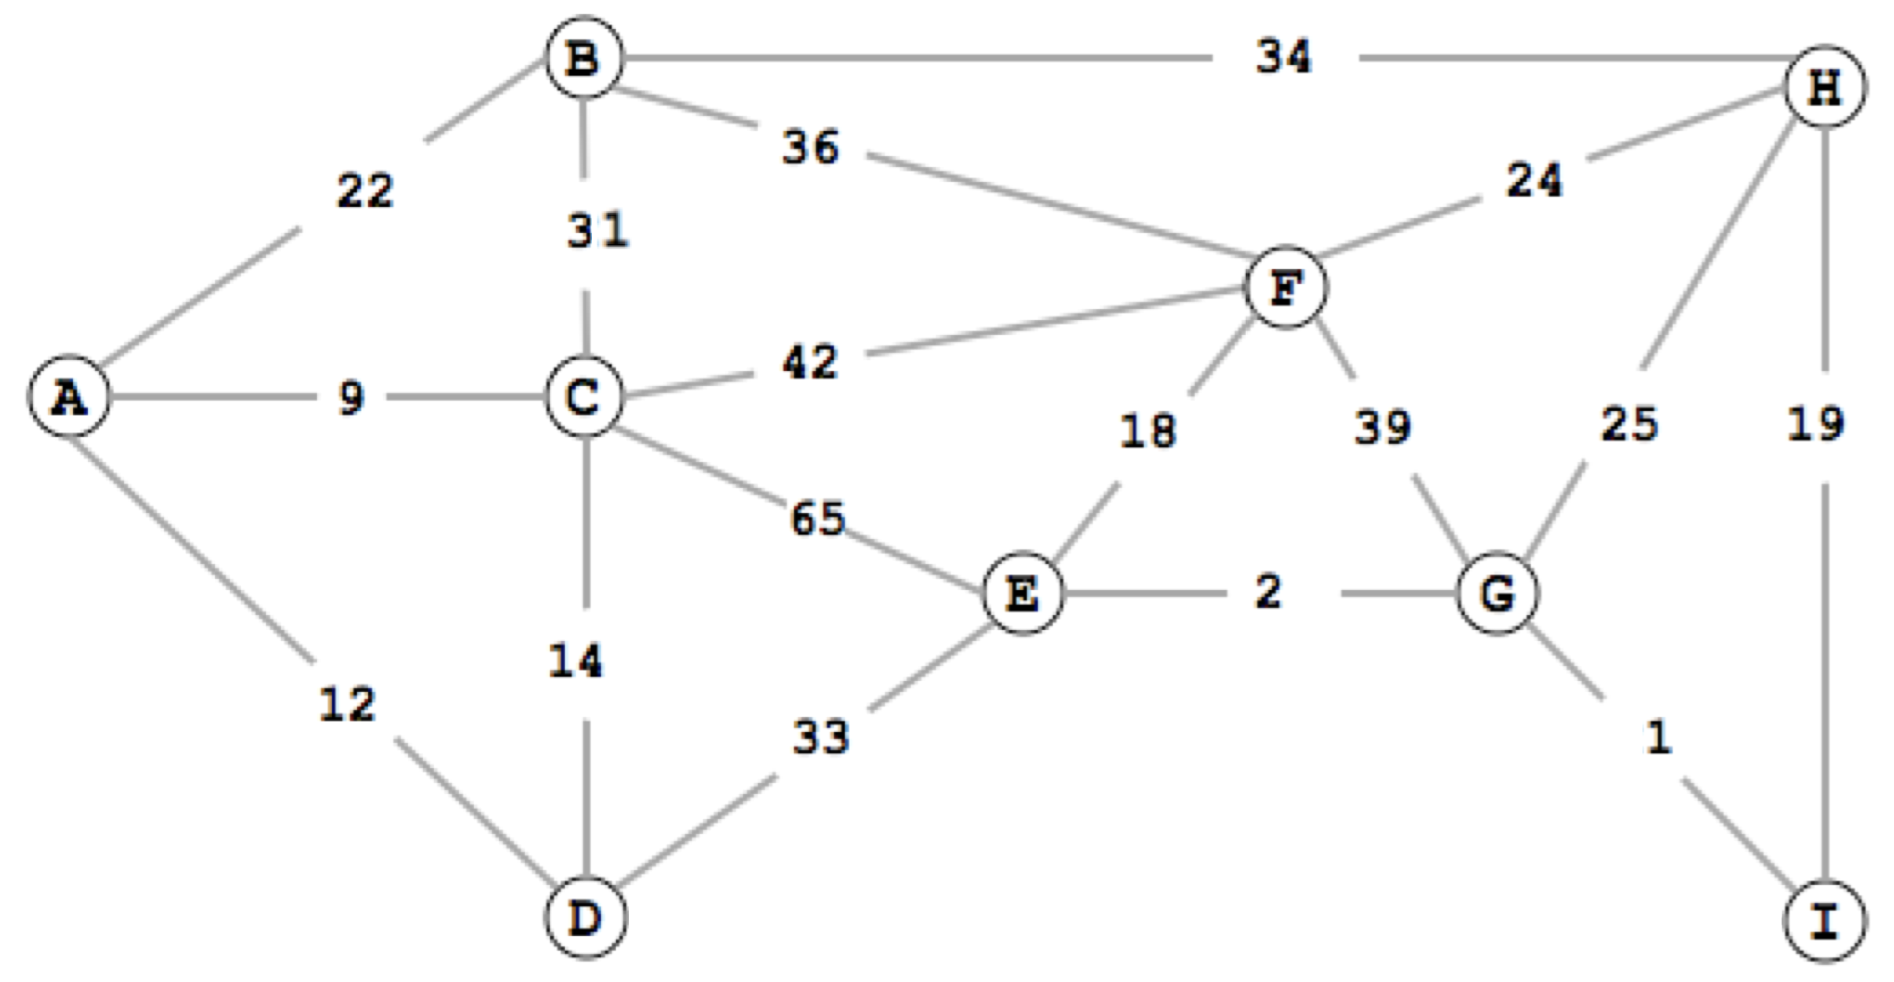
\includegraphics[width=0.8\textwidth]{mst.png}
%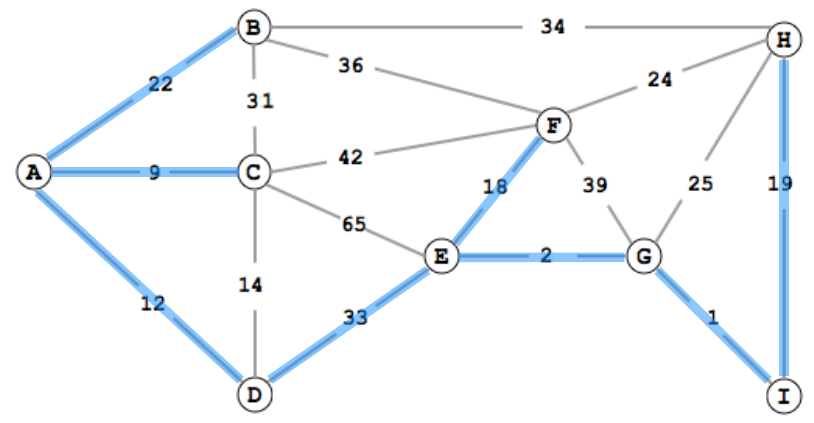
\includegraphics[width=0.8\textwidth]{mstsolution.png}
\end{figure}

\begin{parts}
\part[5] Find the minimum spanning tree of the graph by using Kruskal's algorithm. Highlight the minimum spanning tree edges in the figure above, and list the edges in the order of selection by the algorithm.
\begin{solution}[\stretch{1}]
$GI, EG, AC, AD, EF, HI, AB, DE$
\end{solution}

\part[5] Find the minimum spanning tree of the graph by using Prim's algorithm, starting at node \verb+A+. The same graph is plotted again for your convenience below. List the edges in the order of selection by the algorithm.
\begin{solution}[\stretch{1}]
$AC, AD, AB, DE, EG, GI, EF, HI$
\end{solution}
\begin{figure}[ht!]
\centering
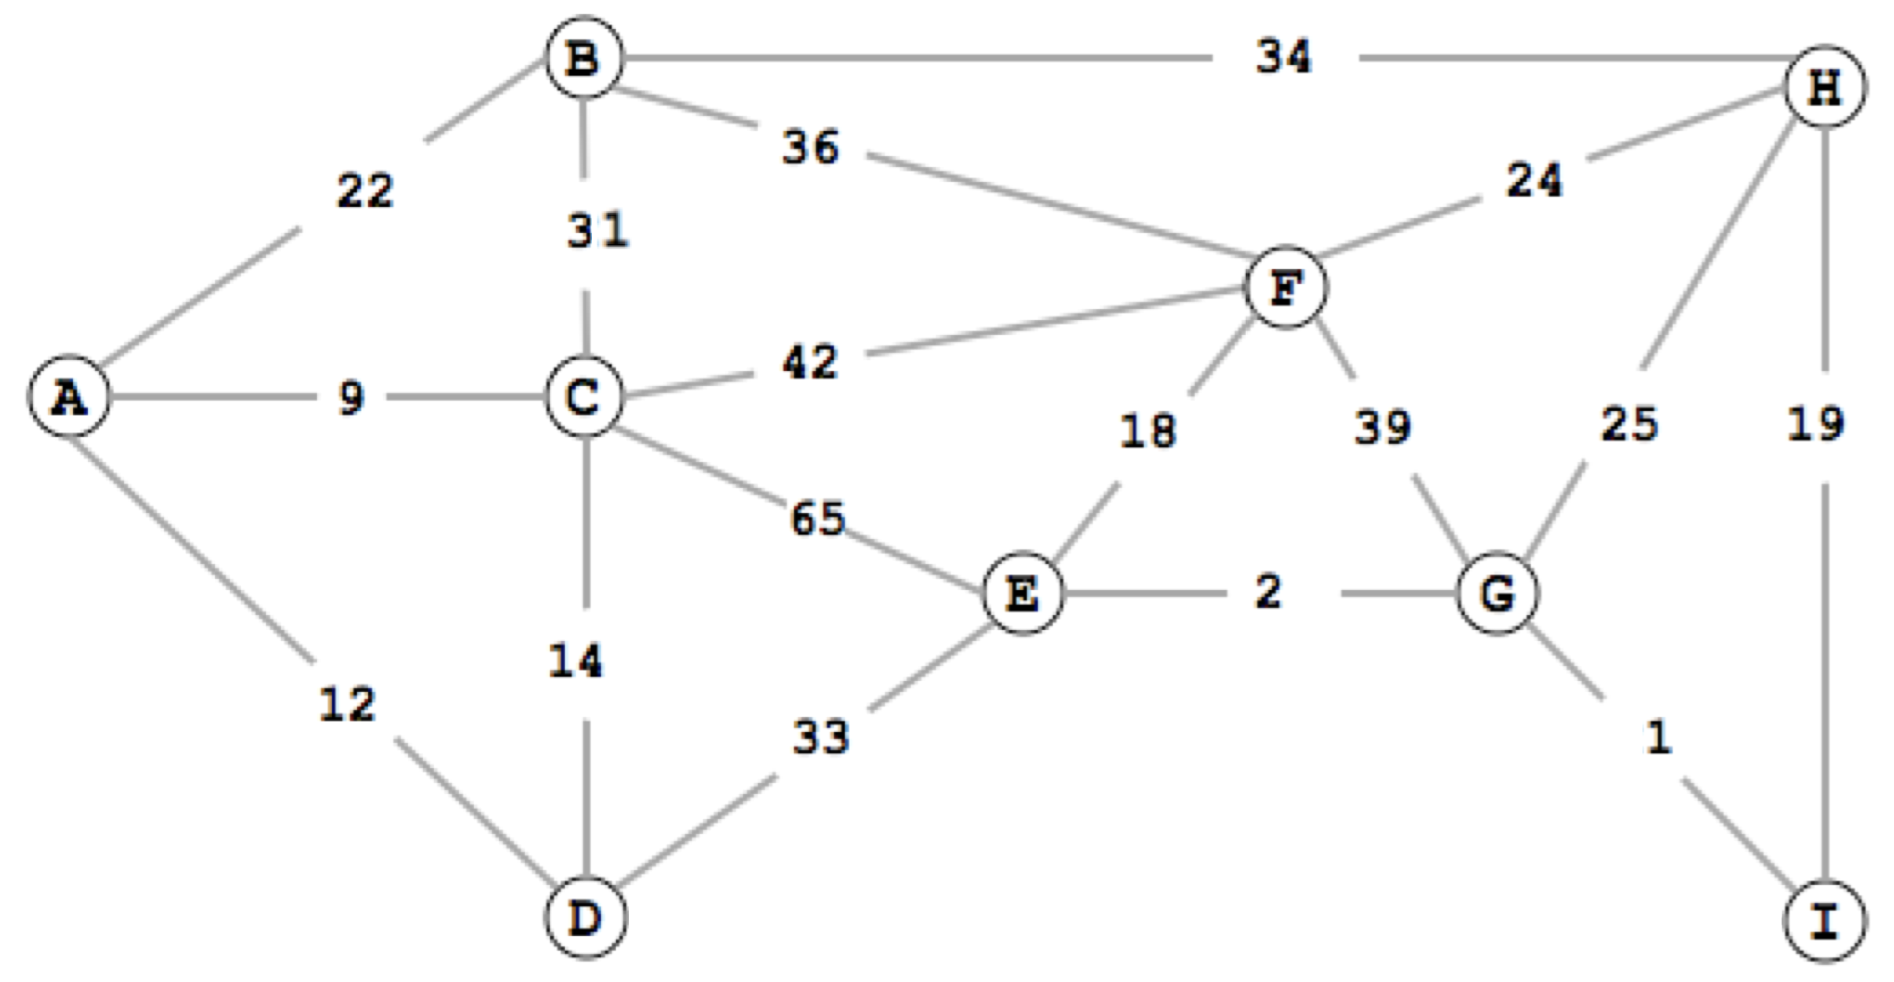
\includegraphics[width=0.8\textwidth]{mst.png}
%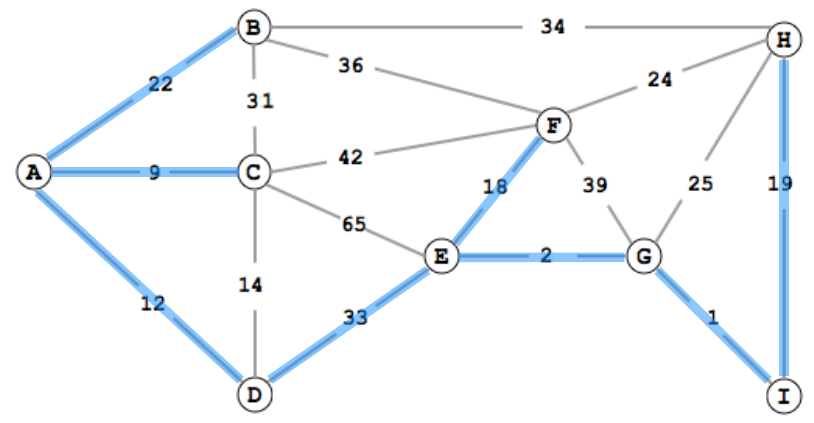
\includegraphics[width=0.8\textwidth]{mstsolution.png}
\end{figure}
\end{parts}




\clearpage
\titledquestion{Command Line Tools} 
Consider working with a UNIX terminal (i.e., the default terminal on a mac or in WSL).\\
In the following, lines starting with \verb+%+ are commands (or pipelines), other lines are outputs.

\begin{parts}

\part
Describe with one or two short sentences each command and its output.
\begin{subparts}
\subpart[1]
\begin{verbatim}

% ssh misz@hpc.itu.dk
Welcome to hpc.itu.dk!
\end{verbatim}
\begin{solution}[\stretch{1}]
Connect to remote server. Welcome message from server.
\end{solution}

\subpart[1] 
\begin{verbatim}

% cd data/
% ls
exam.csv      exam2.csv      raw
\end{verbatim}
\begin{solution}[\stretch{1}]
Switch to directory data, list folder contents.
\end{solution}

\subpart[1] 
\begin{verbatim}

% wc -l exam.csv
5 exam.csv
\end{verbatim}
\begin{solution}[\stretch{1}]
Count the number of lines in file. Show number of lines and filename.
\end{solution}

\end{subparts}


\part
Assume the following command is run with the output shown below it:
\begin{verbatim}
% cat exam.csv
id,grade,points,name
14353,10,86,smith
14233,12,99,vybornova
14533,10,84,pedersen
13633,02,58,szell
\end{verbatim}

\begin{subparts}
\subpart[2] 
What is the output that the following pipeline will generate?
\begin{verbatim}
% head -1 exam.csv | tr "," "\n" | sort | tr "\n" ","
\end{verbatim}
\begin{solution}[\stretch{1}]
\begin{verbatim}
grade,id,name,points,
\end{verbatim}
\end{solution}

\subpart[2] What is the output that the following pipeline will generate? \\Note: \verb+NR>1+ means that the first line is skipped.
\begin{verbatim}
% awk -F',' 'NR>1 {print $2}' exam.csv | sort | uniq | tr "\n" " "
\end{verbatim}
\begin{solution}[\stretch{1}]
\begin{verbatim}
02 10 12
\end{verbatim}
\end{solution}



\subpart[3]
Write a pipeline that creates a new file \verb+names_sorted.txt+ with the following content:
\end{subparts}
\begin{verbatim}
pedersen
smith
szell
vybornova
\end{verbatim}
\begin{solution}[\stretch{2}]
\begin{verbatim}
% awk -F',' 'NR>1 {print $4}' exam.csv | sort > names_sorted.txt
\end{verbatim}
\end{solution}
\end{parts}

\end{questions}

\end{document}